\documentclass[a1,landscape]{a0poster}
\usepackage{etoolbox}
\patchcmd{\thebibliography}{\section*{\refname}}{}{}{}
% \usepackage[margin={5cm,1cm,5cm,5cm}]{geometry}
\usepackage[left=5cm, right=5cm, top=5cm, bottom=0cm]{geometry}
\setlength\textwidth{78cm}
\usepackage[compact]{titlesec}

\usepackage{multicol} % This is so we can have multiple columns of text side-by-side
\columnsep=70pt % This is the amount of white space between the columns in the poster
\columnseprule=3pt % This is the thickness of the black line between the columns in the poster

\usepackage[svgnames]{xcolor} 

\usepackage{times} 

\usepackage{graphicx} % Required for including images
\graphicspath{{figures/}} % Location of the graphics files
\usepackage[font=small,labelfont=bf]{caption} % Required for specifying captions to tables and figures
\usepackage{amsfonts, amsmath, amsthm, amssymb} % For math fonts, symbols and environments
\usepackage{wrapfig} % Allows wrapping text around tables and figures
\usepackage{graphicx}

\begin{document}

\begin{minipage}[c]{0.9\linewidth}
\centering
\Huge \color{NavyBlue} \textbf{Question Answering with 2-Stage Candidate Selection} \color{Black}\\ % Title
\LARGE \textbf{Adam Davies \& Carlos Jimenez}\\ % Author(s)
\end{minipage}

% \vspace{1cm} % A bit of extra whitespace between the header and poster content

%----------------------------------------------------------------------------------------

\begin{multicols}{3} % This is how many columns your poster will be broken into, a poster with many figures may benefit from less columns whereas a text-heavy poster benefits from more
\Large

\color{SaddleBrown} % SaddleBrown color for the introduction

\textbf{\LARGE \\Introduction}\\
\textbf{Our objective} was to design a \textbf{single-document question answering (QA) system}. Our system follows a 2-stage approach: first, candidate sentence selection; second, answer phrase identification. This approach was inspired by that of Wang, Liu, Xiao et al.$^{[1]}$ We began by performing question classification (via constituency parse); next, we used lexical analysis and a rule-based approach for candidate sentence selection; finally, we utilized syntactic argument analysis, guided by dependency/constituency parsing and semantic cues, to produce an answer phrase.

\vspace{1ex}
%----------------------------------------------------------------------------------------
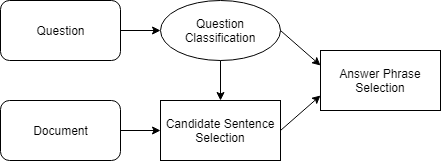
\includegraphics[scale=1.5]{diagram-simple.png}
%----------------------------------------------------------------------------------------

\color{DarkSlateGray} % DarkSlateGray color for the rest of the content

\textbf{\LARGE \\Tools Used}\\
\textbf{Natural Language Tool-Kit (NLTK)}: Used directly for tokenization, lemmatization, POS tagging, some NER, and chunking.\\
\textbf{Stanford CoreNLP}: Accessed via NLTK to provide constituency and dependency parses. \\
\textbf{Gensim, Wordnet}: Both assessed word similarity (Gensim via pre-trained embeddings, Wordnet via `synsets'). \\
\textbf{SpaCy}: Provided some forms of NER and dependency parsing.\\
\textbf{\LARGE Stage 1: Candidate Sentence Selection}\\
Our first stage required question classification into questions types. This enabled us to treat each case differently, and additionally deal with particular sub-cases. \\
For example, if we know we are dealing with a `how-much' type question, we can often identify candidate sentences by those containing MONEY patterns, or CARDINAL entities. After narrowing down the pool of candidates, we filter our candidate pool through more general sentence selection subprocesses. \\
\textbf{The ``general" case:} Our system has two generalized processes to rank candidate sentences.\\ For example, one process involved extracting sentences' lemmatized words, while preserving POS tags, and comparing them with those words in the question processed the same way. Sentences are then ranked by similarity (via Wordnet `synsets' and Gensim's word embeddings), and passed on to the second stage (answer identification).
%------------------------------------------------

\textbf{\LARGE \\Stage 2: Answer Phrase Selection}\\
The second stage began with dependency parsing to determine relevant syntactic arguments (e.g. subject, direct object, etc.). Next, we used Wordnet `synsets', Gensim vector similarity measures, and NER to determine the extent to which various arguments satisfied the semantic properties expected based on the type of question. (For example: `who' questions expected ENTITY types, or words related to `person' or `organization', in subject or direct object positions; `where' questions expected LOCATION types, or words related to various synonyms of `location', as prepositional objects; etc.). \\
Finally, we found the constituents nested within the most relevant arguments (or, in some cases, arguments nested within relevant constituents) of the expected form for the given question-type, and returned it.
\color{SaddleBrown} % SaddleBrown color for the conclusions to make them stand out
\textbf{\LARGE\\Conclusions}\\
\textbf{What Worked Well}
\begin{itemize}
    \item Using a three-pronged approach of NER, word embeddings, and Wordnet `synsets' made sure desired information was almost always captured.
    \item Rule-based additions and heuristics often improved performance significantly, and were easy to implement. 
\end{itemize}
\vspace{0.7em}
\textbf{What Did Not}
\begin{itemize}
    \item Relying too heavily on parsing sometimes resulted in a lack of robustness (given answers occurring in unexpected syntactic structures).
\end{itemize}
\end{multicols}
\color{DarkSlateGray} % Set the color back to DarkSlateGray for the rest of the content
\nocite{*} % Print all references regardless of whether they were cited in the poster or not
\bibliographystyle{plain}
\bibliography{sample.bib}


\end{document}
